\documentclass[twoside]{book}

% Packages required by doxygen
\usepackage{fixltx2e}
\usepackage{calc}
\usepackage{doxygen}
\usepackage[export]{adjustbox} % also loads graphicx
\usepackage{graphicx}
\usepackage[utf8]{inputenc}
\usepackage{makeidx}
\usepackage{multicol}
\usepackage{multirow}
\PassOptionsToPackage{warn}{textcomp}
\usepackage{textcomp}
\usepackage[nointegrals]{wasysym}
\usepackage[table]{xcolor}

% Font selection
\usepackage[T1]{fontenc}
\usepackage[scaled=.90]{helvet}
\usepackage{courier}
\usepackage{amssymb}
\usepackage{sectsty}
\renewcommand{\familydefault}{\sfdefault}
\allsectionsfont{%
  \fontseries{bc}\selectfont%
  \color{darkgray}%
}
\renewcommand{\DoxyLabelFont}{%
  \fontseries{bc}\selectfont%
  \color{darkgray}%
}
\newcommand{\+}{\discretionary{\mbox{\scriptsize$\hookleftarrow$}}{}{}}

% Page & text layout
\usepackage{geometry}
\geometry{%
  a4paper,%
  top=2.5cm,%
  bottom=2.5cm,%
  left=2.5cm,%
  right=2.5cm%
}
\tolerance=750
\hfuzz=15pt
\hbadness=750
\setlength{\emergencystretch}{15pt}
\setlength{\parindent}{0cm}
\setlength{\parskip}{3ex plus 2ex minus 2ex}
\makeatletter
\renewcommand{\paragraph}{%
  \@startsection{paragraph}{4}{0ex}{-1.0ex}{1.0ex}{%
    \normalfont\normalsize\bfseries\SS@parafont%
  }%
}
\renewcommand{\subparagraph}{%
  \@startsection{subparagraph}{5}{0ex}{-1.0ex}{1.0ex}{%
    \normalfont\normalsize\bfseries\SS@subparafont%
  }%
}
\makeatother

% Headers & footers
\usepackage{fancyhdr}
\pagestyle{fancyplain}
\fancyhead[LE]{\fancyplain{}{\bfseries\thepage}}
\fancyhead[CE]{\fancyplain{}{}}
\fancyhead[RE]{\fancyplain{}{\bfseries\leftmark}}
\fancyhead[LO]{\fancyplain{}{\bfseries\rightmark}}
\fancyhead[CO]{\fancyplain{}{}}
\fancyhead[RO]{\fancyplain{}{\bfseries\thepage}}
\fancyfoot[LE]{\fancyplain{}{}}
\fancyfoot[CE]{\fancyplain{}{}}
\fancyfoot[RE]{\fancyplain{}{\bfseries\scriptsize Generated by Doxygen }}
\fancyfoot[LO]{\fancyplain{}{\bfseries\scriptsize Generated by Doxygen }}
\fancyfoot[CO]{\fancyplain{}{}}
\fancyfoot[RO]{\fancyplain{}{}}
\renewcommand{\footrulewidth}{0.4pt}
\renewcommand{\chaptermark}[1]{%
  \markboth{#1}{}%
}
\renewcommand{\sectionmark}[1]{%
  \markright{\thesection\ #1}%
}

% Indices & bibliography
\usepackage{natbib}
\usepackage[titles]{tocloft}
\setcounter{tocdepth}{3}
\setcounter{secnumdepth}{5}
\makeindex

% Hyperlinks (required, but should be loaded last)
\usepackage{ifpdf}
\ifpdf
  \usepackage[pdftex,pagebackref=true]{hyperref}
\else
  \usepackage[ps2pdf,pagebackref=true]{hyperref}
\fi
\hypersetup{%
  colorlinks=true,%
  linkcolor=blue,%
  citecolor=blue,%
  unicode%
}

% Custom commands
\newcommand{\clearemptydoublepage}{%
  \newpage{\pagestyle{empty}\cleardoublepage}%
}

\usepackage{caption}
\captionsetup{labelsep=space,justification=centering,font={bf},singlelinecheck=off,skip=4pt,position=top}

%===== C O N T E N T S =====

\begin{document}

% Titlepage & ToC
\hypersetup{pageanchor=false,
             bookmarksnumbered=true,
             pdfencoding=unicode
            }
\pagenumbering{roman}
\begin{titlepage}
\vspace*{7cm}
\begin{center}%
{\Large Settings\+Package }\\
\vspace*{1cm}
{\large Generated by Doxygen 1.8.11}\\
\end{center}
\end{titlepage}
\clearemptydoublepage
\tableofcontents
\clearemptydoublepage
\pagenumbering{arabic}
\hypersetup{pageanchor=true}

%--- Begin generated contents ---
\chapter{Class Index}
\section{Class List}
Here are the classes, structs, unions and interfaces with brief descriptions\+:\begin{DoxyCompactList}
\item\contentsline{section}{\hyperlink{class_graphics_settings_package}{Graphics\+Settings\+Package} }{\pageref{class_graphics_settings_package}}{}
\item\contentsline{section}{\hyperlink{class_optimizer_settings_package}{Optimizer\+Settings\+Package} }{\pageref{class_optimizer_settings_package}}{}
\item\contentsline{section}{\hyperlink{class_problem_domain_settings_package}{Problem\+Domain\+Settings\+Package} }{\pageref{class_problem_domain_settings_package}}{}
\item\contentsline{section}{\hyperlink{class_settings_package}{Settings\+Package} }{\pageref{class_settings_package}}{}
\end{DoxyCompactList}

\chapter{Class Documentation}
\hypertarget{class_graphics_settings_package}{}\section{Graphics\+Settings\+Package Class Reference}
\label{class_graphics_settings_package}\index{Graphics\+Settings\+Package@{Graphics\+Settings\+Package}}
\subsection*{Public Member Functions}
\begin{DoxyCompactItemize}
\item 
\hyperlink{class_graphics_settings_package_a52641ab244a183d2c77519b21bf33f26}{Graphics\+Settings\+Package} ()\hypertarget{class_graphics_settings_package_a52641ab244a183d2c77519b21bf33f26}{}\label{class_graphics_settings_package_a52641ab244a183d2c77519b21bf33f26}

\begin{DoxyCompactList}\small\item\em The default constructor for an \hyperlink{class_optimizer_settings_package}{Optimizer\+Settings\+Package}. \end{DoxyCompactList}\item 
\hyperlink{class_graphics_settings_package_a09daf855313f3986824a336ee8be7144}{Graphics\+Settings\+Package} (int, int, int, bool, bool, int)
\begin{DoxyCompactList}\small\item\em Creates a \hyperlink{class_graphics_settings_package}{Graphics\+Settings\+Package} with specified settings (currently unused) \end{DoxyCompactList}\item 
int \hyperlink{class_graphics_settings_package_a878709b5b337eeb1ecd41ff36bc3774c}{get\+ResolutionH} ()
\item 
int \hyperlink{class_graphics_settings_package_ae2fbf744672662adde93eaf74c0f3dcf}{get\+ResolutionW} ()
\item 
int \hyperlink{class_graphics_settings_package_ae156dc777c17b698950fb873c427ffeb}{get\+Render\+Speed} ()
\item 
bool \hyperlink{class_graphics_settings_package_a633283a363dcf21db5e4c04d9b79fa2d}{get\+Show\+Links} ()
\item 
bool \hyperlink{class_graphics_settings_package_a4045a81b41cacf97a38212c5a4c65418}{get\+Show\+Path} ()
\item 
int \hyperlink{class_graphics_settings_package_aa6cc824f2ba164264dd79d766f6ed0da}{get\+Max\+Ram} ()
\item 
void \hyperlink{class_graphics_settings_package_a0d9283ca3ba96e9bafeb92f250a71411}{set\+ResolutionH} (int)
\begin{DoxyCompactList}\small\item\em Sets the resolution height. \end{DoxyCompactList}\item 
void \hyperlink{class_graphics_settings_package_a83cc77d7339a3a68dac112c226308a0f}{set\+ResolutionW} (int)
\begin{DoxyCompactList}\small\item\em Sets the resolution width. \end{DoxyCompactList}\item 
void \hyperlink{class_graphics_settings_package_af0e969ea73e1236bcf23cf6ea15e8fa5}{set\+Render\+Speed} (int)
\begin{DoxyCompactList}\small\item\em Sets the render speed. \end{DoxyCompactList}\item 
void \hyperlink{class_graphics_settings_package_a33f4f25bbe31c06e6849abb5c4fb0718}{set\+Show\+Links} (bool)
\begin{DoxyCompactList}\small\item\em Sets link showing on or off. \end{DoxyCompactList}\item 
void \hyperlink{class_graphics_settings_package_a846df7b60107287dac6f795cd1ca7bbb}{set\+Show\+Path} (bool)
\begin{DoxyCompactList}\small\item\em Sets path showing on or off. \end{DoxyCompactList}\item 
void \hyperlink{class_graphics_settings_package_ac84e46d0a2780c49a785c2cfdda6ade8}{set\+Max\+Ram} (int)
\begin{DoxyCompactList}\small\item\em Sets maximum useable ram in megabytes. \end{DoxyCompactList}\end{DoxyCompactItemize}


\subsection{Constructor \& Destructor Documentation}
\index{Graphics\+Settings\+Package@{Graphics\+Settings\+Package}!Graphics\+Settings\+Package@{Graphics\+Settings\+Package}}
\index{Graphics\+Settings\+Package@{Graphics\+Settings\+Package}!Graphics\+Settings\+Package@{Graphics\+Settings\+Package}}
\subsubsection[{\texorpdfstring{Graphics\+Settings\+Package(int, int, int, bool, bool, int)}{GraphicsSettingsPackage(int, int, int, bool, bool, int)}}]{\setlength{\rightskip}{0pt plus 5cm}Graphics\+Settings\+Package\+::\+Graphics\+Settings\+Package (
\begin{DoxyParamCaption}
\item[{int}]{resH, }
\item[{int}]{resW, }
\item[{int}]{rend\+Speed, }
\item[{bool}]{links, }
\item[{bool}]{path, }
\item[{int}]{ram}
\end{DoxyParamCaption}
)}\hypertarget{class_graphics_settings_package_a09daf855313f3986824a336ee8be7144}{}\label{class_graphics_settings_package_a09daf855313f3986824a336ee8be7144}


Creates a \hyperlink{class_graphics_settings_package}{Graphics\+Settings\+Package} with specified settings (currently unused) 


\begin{DoxyParams}{Parameters}
{\em Resolution} & height (int) \\
\hline
{\em Resolution} & width (int) \\
\hline
{\em Render} & speed (int) \\
\hline
{\em Show\+Links(bool)} & \\
\hline
{\em Show\+Path} & (bool) \\
\hline
{\em Max\+Ram} & (int) \\
\hline
\end{DoxyParams}


\subsection{Member Function Documentation}
\index{Graphics\+Settings\+Package@{Graphics\+Settings\+Package}!get\+Max\+Ram@{get\+Max\+Ram}}
\index{get\+Max\+Ram@{get\+Max\+Ram}!Graphics\+Settings\+Package@{Graphics\+Settings\+Package}}
\subsubsection[{\texorpdfstring{get\+Max\+Ram()}{getMaxRam()}}]{\setlength{\rightskip}{0pt plus 5cm}int Graphics\+Settings\+Package\+::get\+Max\+Ram (
\begin{DoxyParamCaption}
{}
\end{DoxyParamCaption}
)}\hypertarget{class_graphics_settings_package_aa6cc824f2ba164264dd79d766f6ed0da}{}\label{class_graphics_settings_package_aa6cc824f2ba164264dd79d766f6ed0da}
\begin{DoxyReturn}{Returns}
Returns the max useable ram in Megabytes (an int) 
\end{DoxyReturn}
\index{Graphics\+Settings\+Package@{Graphics\+Settings\+Package}!get\+Render\+Speed@{get\+Render\+Speed}}
\index{get\+Render\+Speed@{get\+Render\+Speed}!Graphics\+Settings\+Package@{Graphics\+Settings\+Package}}
\subsubsection[{\texorpdfstring{get\+Render\+Speed()}{getRenderSpeed()}}]{\setlength{\rightskip}{0pt plus 5cm}int Graphics\+Settings\+Package\+::get\+Render\+Speed (
\begin{DoxyParamCaption}
{}
\end{DoxyParamCaption}
)}\hypertarget{class_graphics_settings_package_ae156dc777c17b698950fb873c427ffeb}{}\label{class_graphics_settings_package_ae156dc777c17b698950fb873c427ffeb}
\begin{DoxyReturn}{Returns}
Returns the render speed (an int) 
\end{DoxyReturn}
\index{Graphics\+Settings\+Package@{Graphics\+Settings\+Package}!get\+ResolutionH@{get\+ResolutionH}}
\index{get\+ResolutionH@{get\+ResolutionH}!Graphics\+Settings\+Package@{Graphics\+Settings\+Package}}
\subsubsection[{\texorpdfstring{get\+Resolution\+H()}{getResolutionH()}}]{\setlength{\rightskip}{0pt plus 5cm}int Graphics\+Settings\+Package\+::get\+ResolutionH (
\begin{DoxyParamCaption}
{}
\end{DoxyParamCaption}
)}\hypertarget{class_graphics_settings_package_a878709b5b337eeb1ecd41ff36bc3774c}{}\label{class_graphics_settings_package_a878709b5b337eeb1ecd41ff36bc3774c}
\begin{DoxyReturn}{Returns}
Returns the resolution height dimension (an int) 
\end{DoxyReturn}
\index{Graphics\+Settings\+Package@{Graphics\+Settings\+Package}!get\+ResolutionW@{get\+ResolutionW}}
\index{get\+ResolutionW@{get\+ResolutionW}!Graphics\+Settings\+Package@{Graphics\+Settings\+Package}}
\subsubsection[{\texorpdfstring{get\+Resolution\+W()}{getResolutionW()}}]{\setlength{\rightskip}{0pt plus 5cm}int Graphics\+Settings\+Package\+::get\+ResolutionW (
\begin{DoxyParamCaption}
{}
\end{DoxyParamCaption}
)}\hypertarget{class_graphics_settings_package_ae2fbf744672662adde93eaf74c0f3dcf}{}\label{class_graphics_settings_package_ae2fbf744672662adde93eaf74c0f3dcf}
\begin{DoxyReturn}{Returns}
Returns the resolution width dimension (an int) 
\end{DoxyReturn}
\index{Graphics\+Settings\+Package@{Graphics\+Settings\+Package}!get\+Show\+Links@{get\+Show\+Links}}
\index{get\+Show\+Links@{get\+Show\+Links}!Graphics\+Settings\+Package@{Graphics\+Settings\+Package}}
\subsubsection[{\texorpdfstring{get\+Show\+Links()}{getShowLinks()}}]{\setlength{\rightskip}{0pt plus 5cm}bool Graphics\+Settings\+Package\+::get\+Show\+Links (
\begin{DoxyParamCaption}
{}
\end{DoxyParamCaption}
)}\hypertarget{class_graphics_settings_package_a633283a363dcf21db5e4c04d9b79fa2d}{}\label{class_graphics_settings_package_a633283a363dcf21db5e4c04d9b79fa2d}
\begin{DoxyReturn}{Returns}
Returns whether links are to be shown or not (a bool) 
\end{DoxyReturn}
\index{Graphics\+Settings\+Package@{Graphics\+Settings\+Package}!get\+Show\+Path@{get\+Show\+Path}}
\index{get\+Show\+Path@{get\+Show\+Path}!Graphics\+Settings\+Package@{Graphics\+Settings\+Package}}
\subsubsection[{\texorpdfstring{get\+Show\+Path()}{getShowPath()}}]{\setlength{\rightskip}{0pt plus 5cm}bool Graphics\+Settings\+Package\+::get\+Show\+Path (
\begin{DoxyParamCaption}
{}
\end{DoxyParamCaption}
)}\hypertarget{class_graphics_settings_package_a4045a81b41cacf97a38212c5a4c65418}{}\label{class_graphics_settings_package_a4045a81b41cacf97a38212c5a4c65418}
\begin{DoxyReturn}{Returns}
Returns whether the path is shown or not (a bool) 
\end{DoxyReturn}
\index{Graphics\+Settings\+Package@{Graphics\+Settings\+Package}!set\+Max\+Ram@{set\+Max\+Ram}}
\index{set\+Max\+Ram@{set\+Max\+Ram}!Graphics\+Settings\+Package@{Graphics\+Settings\+Package}}
\subsubsection[{\texorpdfstring{set\+Max\+Ram(int)}{setMaxRam(int)}}]{\setlength{\rightskip}{0pt plus 5cm}void Graphics\+Settings\+Package\+::set\+Max\+Ram (
\begin{DoxyParamCaption}
\item[{int}]{new\+Ram}
\end{DoxyParamCaption}
)}\hypertarget{class_graphics_settings_package_ac84e46d0a2780c49a785c2cfdda6ade8}{}\label{class_graphics_settings_package_ac84e46d0a2780c49a785c2cfdda6ade8}


Sets maximum useable ram in megabytes. 


\begin{DoxyParams}{Parameters}
{\em Max\+Ram} & (int) \\
\hline
\end{DoxyParams}
\index{Graphics\+Settings\+Package@{Graphics\+Settings\+Package}!set\+Render\+Speed@{set\+Render\+Speed}}
\index{set\+Render\+Speed@{set\+Render\+Speed}!Graphics\+Settings\+Package@{Graphics\+Settings\+Package}}
\subsubsection[{\texorpdfstring{set\+Render\+Speed(int)}{setRenderSpeed(int)}}]{\setlength{\rightskip}{0pt plus 5cm}void Graphics\+Settings\+Package\+::set\+Render\+Speed (
\begin{DoxyParamCaption}
\item[{int}]{new\+Rend}
\end{DoxyParamCaption}
)}\hypertarget{class_graphics_settings_package_af0e969ea73e1236bcf23cf6ea15e8fa5}{}\label{class_graphics_settings_package_af0e969ea73e1236bcf23cf6ea15e8fa5}


Sets the render speed. 


\begin{DoxyParams}{Parameters}
{\em Render\+Speed} & (int) \\
\hline
\end{DoxyParams}
\index{Graphics\+Settings\+Package@{Graphics\+Settings\+Package}!set\+ResolutionH@{set\+ResolutionH}}
\index{set\+ResolutionH@{set\+ResolutionH}!Graphics\+Settings\+Package@{Graphics\+Settings\+Package}}
\subsubsection[{\texorpdfstring{set\+Resolution\+H(int)}{setResolutionH(int)}}]{\setlength{\rightskip}{0pt plus 5cm}void Graphics\+Settings\+Package\+::set\+ResolutionH (
\begin{DoxyParamCaption}
\item[{int}]{newH}
\end{DoxyParamCaption}
)}\hypertarget{class_graphics_settings_package_a0d9283ca3ba96e9bafeb92f250a71411}{}\label{class_graphics_settings_package_a0d9283ca3ba96e9bafeb92f250a71411}


Sets the resolution height. 


\begin{DoxyParams}{Parameters}
{\em Resolution\+Height} & (int) \\
\hline
\end{DoxyParams}
\index{Graphics\+Settings\+Package@{Graphics\+Settings\+Package}!set\+ResolutionW@{set\+ResolutionW}}
\index{set\+ResolutionW@{set\+ResolutionW}!Graphics\+Settings\+Package@{Graphics\+Settings\+Package}}
\subsubsection[{\texorpdfstring{set\+Resolution\+W(int)}{setResolutionW(int)}}]{\setlength{\rightskip}{0pt plus 5cm}void Graphics\+Settings\+Package\+::set\+ResolutionW (
\begin{DoxyParamCaption}
\item[{int}]{newW}
\end{DoxyParamCaption}
)}\hypertarget{class_graphics_settings_package_a83cc77d7339a3a68dac112c226308a0f}{}\label{class_graphics_settings_package_a83cc77d7339a3a68dac112c226308a0f}


Sets the resolution width. 


\begin{DoxyParams}{Parameters}
{\em Resolution\+Width} & (int) \\
\hline
\end{DoxyParams}
\index{Graphics\+Settings\+Package@{Graphics\+Settings\+Package}!set\+Show\+Links@{set\+Show\+Links}}
\index{set\+Show\+Links@{set\+Show\+Links}!Graphics\+Settings\+Package@{Graphics\+Settings\+Package}}
\subsubsection[{\texorpdfstring{set\+Show\+Links(bool)}{setShowLinks(bool)}}]{\setlength{\rightskip}{0pt plus 5cm}void Graphics\+Settings\+Package\+::set\+Show\+Links (
\begin{DoxyParamCaption}
\item[{bool}]{links}
\end{DoxyParamCaption}
)}\hypertarget{class_graphics_settings_package_a33f4f25bbe31c06e6849abb5c4fb0718}{}\label{class_graphics_settings_package_a33f4f25bbe31c06e6849abb5c4fb0718}


Sets link showing on or off. 


\begin{DoxyParams}{Parameters}
{\em Show\+Link} & (bool) \\
\hline
\end{DoxyParams}
\index{Graphics\+Settings\+Package@{Graphics\+Settings\+Package}!set\+Show\+Path@{set\+Show\+Path}}
\index{set\+Show\+Path@{set\+Show\+Path}!Graphics\+Settings\+Package@{Graphics\+Settings\+Package}}
\subsubsection[{\texorpdfstring{set\+Show\+Path(bool)}{setShowPath(bool)}}]{\setlength{\rightskip}{0pt plus 5cm}void Graphics\+Settings\+Package\+::set\+Show\+Path (
\begin{DoxyParamCaption}
\item[{bool}]{path}
\end{DoxyParamCaption}
)}\hypertarget{class_graphics_settings_package_a846df7b60107287dac6f795cd1ca7bbb}{}\label{class_graphics_settings_package_a846df7b60107287dac6f795cd1ca7bbb}


Sets path showing on or off. 


\begin{DoxyParams}{Parameters}
{\em Show\+Path} & (bool) \\
\hline
\end{DoxyParams}


The documentation for this class was generated from the following files\+:\begin{DoxyCompactItemize}
\item 
C\+:/\+Users/rento/\+Documents/\+Dragon\+Brain/\+Settings\+Package/src/graphicssettingspackage.\+h\item 
C\+:/\+Users/rento/\+Documents/\+Dragon\+Brain/\+Settings\+Package/src/graphicssettingspackage.\+cpp\end{DoxyCompactItemize}

\hypertarget{class_optimizer_settings_package}{}\section{Optimizer\+Settings\+Package Class Reference}
\label{class_optimizer_settings_package}\index{Optimizer\+Settings\+Package@{Optimizer\+Settings\+Package}}


{\ttfamily \#include $<$graphicssettingspackage.\+h$>$}

\subsection*{Public Member Functions}
\begin{DoxyCompactItemize}
\item 
\hyperlink{class_optimizer_settings_package_a9562747ebfbde1cbda03fee425d886af}{Optimizer\+Settings\+Package} ()\hypertarget{class_optimizer_settings_package_a9562747ebfbde1cbda03fee425d886af}{}\label{class_optimizer_settings_package_a9562747ebfbde1cbda03fee425d886af}

\begin{DoxyCompactList}\small\item\em The default constructor for an \hyperlink{class_optimizer_settings_package}{Optimizer\+Settings\+Package}. \end{DoxyCompactList}\item 
\hyperlink{class_optimizer_settings_package_a69a8c18448ba70702fc6fa3dd87848b4}{Optimizer\+Settings\+Package} (std\+::string $\ast$, double, double, double)
\begin{DoxyCompactList}\small\item\em Creates a \hyperlink{class_optimizer_settings_package}{Optimizer\+Settings\+Package} with specified settings (currently unused) \end{DoxyCompactList}\item 
std\+::string $\ast$ \hyperlink{class_optimizer_settings_package_abbc65564f1d7fae597e36f64c0ba4846}{get\+Particle\+Placement\+String} ()
\item 
double \hyperlink{class_optimizer_settings_package_af914190cf768d01151748918824caadc}{get\+Inertia\+Weight} ()
\item 
double \hyperlink{class_optimizer_settings_package_af760320d4abd50d7202d174064c0081d}{get\+Cognitive\+Coefficient} ()
\item 
double \hyperlink{class_optimizer_settings_package_a1c9c6216fdc974d98240a0ed5a935ab5}{get\+Social\+Coefficient} ()
\item 
void \hyperlink{class_optimizer_settings_package_ae0b23faba2bbc26bd43b2a39077524cf}{set\+Particle\+Placement\+String} (std\+::string $\ast$)
\begin{DoxyCompactList}\small\item\em Sets the Particle Placement. \end{DoxyCompactList}\item 
void \hyperlink{class_optimizer_settings_package_a00f4ac2ec3d1b11b2c0c056dc20e902b}{set\+Inertia\+Weight} (double)
\begin{DoxyCompactList}\small\item\em Sets the Inertia Weight. \end{DoxyCompactList}\item 
void \hyperlink{class_optimizer_settings_package_a5af2e5d9a2b5f7f344e7f840b609c33f}{set\+Cognitive\+Coefficient} (double)
\begin{DoxyCompactList}\small\item\em Sets the Cognitive Coefficient. \end{DoxyCompactList}\item 
void \hyperlink{class_optimizer_settings_package_aa45136551d680be4eca1f647c327e79f}{set\+Social\+Coefficient} (double)
\begin{DoxyCompactList}\small\item\em Sets the Social Coefficient. \end{DoxyCompactList}\end{DoxyCompactItemize}


\subsection{Detailed Description}
This class is a wrapper for all the settings related to the Graphics Processor The contents are rather simplistic, only getters and setters.

This class is a wrapper for all the settings related to the Optimizer The contents are rather simplistic, only getters and setters. 

\subsection{Constructor \& Destructor Documentation}
\index{Optimizer\+Settings\+Package@{Optimizer\+Settings\+Package}!Optimizer\+Settings\+Package@{Optimizer\+Settings\+Package}}
\index{Optimizer\+Settings\+Package@{Optimizer\+Settings\+Package}!Optimizer\+Settings\+Package@{Optimizer\+Settings\+Package}}
\subsubsection[{\texorpdfstring{Optimizer\+Settings\+Package(std\+::string $\ast$, double, double, double)}{OptimizerSettingsPackage(std::string *, double, double, double)}}]{\setlength{\rightskip}{0pt plus 5cm}Optimizer\+Settings\+Package\+::\+Optimizer\+Settings\+Package (
\begin{DoxyParamCaption}
\item[{std\+::string $\ast$}]{particles, }
\item[{double}]{inertia, }
\item[{double}]{cogn, }
\item[{double}]{social}
\end{DoxyParamCaption}
)}\hypertarget{class_optimizer_settings_package_a69a8c18448ba70702fc6fa3dd87848b4}{}\label{class_optimizer_settings_package_a69a8c18448ba70702fc6fa3dd87848b4}


Creates a \hyperlink{class_optimizer_settings_package}{Optimizer\+Settings\+Package} with specified settings (currently unused) 


\begin{DoxyParams}{Parameters}
{\em particle\+Placement} & (string pointer) \\
\hline
{\em inertia\+Weight} & (double) \\
\hline
{\em cognitive\+Coefficient} & (double) \\
\hline
{\em social\+Coefficient} & (double) \\
\hline
\end{DoxyParams}


\subsection{Member Function Documentation}
\index{Optimizer\+Settings\+Package@{Optimizer\+Settings\+Package}!get\+Cognitive\+Coefficient@{get\+Cognitive\+Coefficient}}
\index{get\+Cognitive\+Coefficient@{get\+Cognitive\+Coefficient}!Optimizer\+Settings\+Package@{Optimizer\+Settings\+Package}}
\subsubsection[{\texorpdfstring{get\+Cognitive\+Coefficient()}{getCognitiveCoefficient()}}]{\setlength{\rightskip}{0pt plus 5cm}double Optimizer\+Settings\+Package\+::get\+Cognitive\+Coefficient (
\begin{DoxyParamCaption}
{}
\end{DoxyParamCaption}
)}\hypertarget{class_optimizer_settings_package_af760320d4abd50d7202d174064c0081d}{}\label{class_optimizer_settings_package_af760320d4abd50d7202d174064c0081d}
\begin{DoxyReturn}{Returns}
Returns a double containing the cognitive coefficient 
\end{DoxyReturn}
\index{Optimizer\+Settings\+Package@{Optimizer\+Settings\+Package}!get\+Inertia\+Weight@{get\+Inertia\+Weight}}
\index{get\+Inertia\+Weight@{get\+Inertia\+Weight}!Optimizer\+Settings\+Package@{Optimizer\+Settings\+Package}}
\subsubsection[{\texorpdfstring{get\+Inertia\+Weight()}{getInertiaWeight()}}]{\setlength{\rightskip}{0pt plus 5cm}double Optimizer\+Settings\+Package\+::get\+Inertia\+Weight (
\begin{DoxyParamCaption}
{}
\end{DoxyParamCaption}
)}\hypertarget{class_optimizer_settings_package_af914190cf768d01151748918824caadc}{}\label{class_optimizer_settings_package_af914190cf768d01151748918824caadc}
\begin{DoxyReturn}{Returns}
Returns a double containing the inertia weight 
\end{DoxyReturn}
\index{Optimizer\+Settings\+Package@{Optimizer\+Settings\+Package}!get\+Particle\+Placement\+String@{get\+Particle\+Placement\+String}}
\index{get\+Particle\+Placement\+String@{get\+Particle\+Placement\+String}!Optimizer\+Settings\+Package@{Optimizer\+Settings\+Package}}
\subsubsection[{\texorpdfstring{get\+Particle\+Placement\+String()}{getParticlePlacementString()}}]{\setlength{\rightskip}{0pt plus 5cm}std\+::string $\ast$ Optimizer\+Settings\+Package\+::get\+Particle\+Placement\+String (
\begin{DoxyParamCaption}
{}
\end{DoxyParamCaption}
)}\hypertarget{class_optimizer_settings_package_abbc65564f1d7fae597e36f64c0ba4846}{}\label{class_optimizer_settings_package_abbc65564f1d7fae597e36f64c0ba4846}
\begin{DoxyReturn}{Returns}
Returns the string containing the user specified particle placement (or null) 
\end{DoxyReturn}
\index{Optimizer\+Settings\+Package@{Optimizer\+Settings\+Package}!get\+Social\+Coefficient@{get\+Social\+Coefficient}}
\index{get\+Social\+Coefficient@{get\+Social\+Coefficient}!Optimizer\+Settings\+Package@{Optimizer\+Settings\+Package}}
\subsubsection[{\texorpdfstring{get\+Social\+Coefficient()}{getSocialCoefficient()}}]{\setlength{\rightskip}{0pt plus 5cm}double Optimizer\+Settings\+Package\+::get\+Social\+Coefficient (
\begin{DoxyParamCaption}
{}
\end{DoxyParamCaption}
)}\hypertarget{class_optimizer_settings_package_a1c9c6216fdc974d98240a0ed5a935ab5}{}\label{class_optimizer_settings_package_a1c9c6216fdc974d98240a0ed5a935ab5}
\begin{DoxyReturn}{Returns}
Returns a double containing the social coefficient 
\end{DoxyReturn}
\index{Optimizer\+Settings\+Package@{Optimizer\+Settings\+Package}!set\+Cognitive\+Coefficient@{set\+Cognitive\+Coefficient}}
\index{set\+Cognitive\+Coefficient@{set\+Cognitive\+Coefficient}!Optimizer\+Settings\+Package@{Optimizer\+Settings\+Package}}
\subsubsection[{\texorpdfstring{set\+Cognitive\+Coefficient(double)}{setCognitiveCoefficient(double)}}]{\setlength{\rightskip}{0pt plus 5cm}void Optimizer\+Settings\+Package\+::set\+Cognitive\+Coefficient (
\begin{DoxyParamCaption}
\item[{double}]{cogn}
\end{DoxyParamCaption}
)}\hypertarget{class_optimizer_settings_package_a5af2e5d9a2b5f7f344e7f840b609c33f}{}\label{class_optimizer_settings_package_a5af2e5d9a2b5f7f344e7f840b609c33f}


Sets the Cognitive Coefficient. 


\begin{DoxyParams}{Parameters}
{\em cognitive\+Coefficient} & (double) \\
\hline
\end{DoxyParams}
\index{Optimizer\+Settings\+Package@{Optimizer\+Settings\+Package}!set\+Inertia\+Weight@{set\+Inertia\+Weight}}
\index{set\+Inertia\+Weight@{set\+Inertia\+Weight}!Optimizer\+Settings\+Package@{Optimizer\+Settings\+Package}}
\subsubsection[{\texorpdfstring{set\+Inertia\+Weight(double)}{setInertiaWeight(double)}}]{\setlength{\rightskip}{0pt plus 5cm}void Optimizer\+Settings\+Package\+::set\+Inertia\+Weight (
\begin{DoxyParamCaption}
\item[{double}]{inertia}
\end{DoxyParamCaption}
)}\hypertarget{class_optimizer_settings_package_a00f4ac2ec3d1b11b2c0c056dc20e902b}{}\label{class_optimizer_settings_package_a00f4ac2ec3d1b11b2c0c056dc20e902b}


Sets the Inertia Weight. 


\begin{DoxyParams}{Parameters}
{\em Inertia\+Weight} & (double) \\
\hline
\end{DoxyParams}
\index{Optimizer\+Settings\+Package@{Optimizer\+Settings\+Package}!set\+Particle\+Placement\+String@{set\+Particle\+Placement\+String}}
\index{set\+Particle\+Placement\+String@{set\+Particle\+Placement\+String}!Optimizer\+Settings\+Package@{Optimizer\+Settings\+Package}}
\subsubsection[{\texorpdfstring{set\+Particle\+Placement\+String(std\+::string $\ast$)}{setParticlePlacementString(std::string *)}}]{\setlength{\rightskip}{0pt plus 5cm}void Optimizer\+Settings\+Package\+::set\+Particle\+Placement\+String (
\begin{DoxyParamCaption}
\item[{std\+::string $\ast$}]{particle\+String}
\end{DoxyParamCaption}
)}\hypertarget{class_optimizer_settings_package_ae0b23faba2bbc26bd43b2a39077524cf}{}\label{class_optimizer_settings_package_ae0b23faba2bbc26bd43b2a39077524cf}


Sets the Particle Placement. 


\begin{DoxyParams}{Parameters}
{\em Particle\+Placement} & (string pointer) \\
\hline
\end{DoxyParams}
\index{Optimizer\+Settings\+Package@{Optimizer\+Settings\+Package}!set\+Social\+Coefficient@{set\+Social\+Coefficient}}
\index{set\+Social\+Coefficient@{set\+Social\+Coefficient}!Optimizer\+Settings\+Package@{Optimizer\+Settings\+Package}}
\subsubsection[{\texorpdfstring{set\+Social\+Coefficient(double)}{setSocialCoefficient(double)}}]{\setlength{\rightskip}{0pt plus 5cm}void Optimizer\+Settings\+Package\+::set\+Social\+Coefficient (
\begin{DoxyParamCaption}
\item[{double}]{social}
\end{DoxyParamCaption}
)}\hypertarget{class_optimizer_settings_package_aa45136551d680be4eca1f647c327e79f}{}\label{class_optimizer_settings_package_aa45136551d680be4eca1f647c327e79f}


Sets the Social Coefficient. 


\begin{DoxyParams}{Parameters}
{\em social\+Coefficient} & (double) \\
\hline
\end{DoxyParams}


The documentation for this class was generated from the following files\+:\begin{DoxyCompactItemize}
\item 
Settings\+Package/optimizersettingspackage.\+h\item 
Settings\+Package/optimizersettingspackage.\+cpp\end{DoxyCompactItemize}

\hypertarget{class_problem_domain_settings_package}{}\section{Problem\+Domain\+Settings\+Package Class Reference}
\label{class_problem_domain_settings_package}\index{Problem\+Domain\+Settings\+Package@{Problem\+Domain\+Settings\+Package}}


{\ttfamily \#include $<$problemdomainsettingspackage.\+h$>$}

\subsection*{Public Member Functions}
\begin{DoxyCompactItemize}
\item 
\hyperlink{class_problem_domain_settings_package_acba5f13f17058d9182f23f7e79dfdb53}{Problem\+Domain\+Settings\+Package} ()\hypertarget{class_problem_domain_settings_package_acba5f13f17058d9182f23f7e79dfdb53}{}\label{class_problem_domain_settings_package_acba5f13f17058d9182f23f7e79dfdb53}

\begin{DoxyCompactList}\small\item\em The default constructor for a \hyperlink{class_problem_domain_settings_package}{Problem\+Domain\+Settings\+Package}. \end{DoxyCompactList}\item 
\hyperlink{class_problem_domain_settings_package_ab2c7252d5998c4b2d77f1dca25d030e3}{Problem\+Domain\+Settings\+Package} (std\+::string, int, int\mbox{[}4\mbox{]}, double\mbox{[}3\mbox{]})
\begin{DoxyCompactList}\small\item\em Creates a \hyperlink{class_problem_domain_settings_package}{Problem\+Domain\+Settings\+Package} with specified settings (currently unused) \end{DoxyCompactList}\item 
std\+::string \hyperlink{class_problem_domain_settings_package_a858c5f6501fe46a6469422ca87cbc227}{get\+Objective\+Function} ()
\item 
int \hyperlink{class_problem_domain_settings_package_a1ff00f66433a26e87176915159207a53}{get\+Dimensions} ()
\item 
void \hyperlink{class_problem_domain_settings_package_a004beb40525bd9254a1e9cbb60aac7c9}{get\+Boundaries} (int in\+Array\mbox{[}4\mbox{]})
\begin{DoxyCompactList}\small\item\em Takes an array in and copies the boundary array into it. \end{DoxyCompactList}\item 
void \hyperlink{class_problem_domain_settings_package_a354779476d267a4a5cc39c55c6655a14}{get\+Transformations} (double in\+Array\mbox{[}3\mbox{]})
\begin{DoxyCompactList}\small\item\em Takes an array in and copies the transformations array into it. \end{DoxyCompactList}\item 
void \hyperlink{class_problem_domain_settings_package_ad08819f63bb7d05409489ba9c6049f92}{set\+Objective\+Function} (std\+::string in\+ObjF)
\begin{DoxyCompactList}\small\item\em Sets the objective function. \end{DoxyCompactList}\item 
void \hyperlink{class_problem_domain_settings_package_a99993d6577bd93023adb2cdad0443069}{set\+Dimensions} (int)
\begin{DoxyCompactList}\small\item\em Sets the number of dimensions for the problem. \end{DoxyCompactList}\item 
void \hyperlink{class_problem_domain_settings_package_ac619791d99b6e9bfea96329605997140}{set\+Boundaries} (int\mbox{[}4\mbox{]})
\begin{DoxyCompactList}\small\item\em Sets the boundary values for the dimensions. \end{DoxyCompactList}\item 
void \hyperlink{class_problem_domain_settings_package_ab4f9e9f0656b341549e9e555069735a2}{set\+Transformations} (double\mbox{[}3\mbox{]})
\begin{DoxyCompactList}\small\item\em Sets the transformation values for the problem. \end{DoxyCompactList}\end{DoxyCompactItemize}


\subsection{Detailed Description}
This class is a wrapper for all the settings related to the problem Domain The contents are rather simplistic, only getters and setters.

This class is a general \hyperlink{class_settings_package}{Settings\+Package} which contains other, more specific Settings\+Packages and extracts settings from the G\+UI 

\subsection{Constructor \& Destructor Documentation}
\index{Problem\+Domain\+Settings\+Package@{Problem\+Domain\+Settings\+Package}!Problem\+Domain\+Settings\+Package@{Problem\+Domain\+Settings\+Package}}
\index{Problem\+Domain\+Settings\+Package@{Problem\+Domain\+Settings\+Package}!Problem\+Domain\+Settings\+Package@{Problem\+Domain\+Settings\+Package}}
\subsubsection[{\texorpdfstring{Problem\+Domain\+Settings\+Package(std\+::string, int, int[4], double[3])}{ProblemDomainSettingsPackage(std::string, int, int[4], double[3])}}]{\setlength{\rightskip}{0pt plus 5cm}Problem\+Domain\+Settings\+Package\+::\+Problem\+Domain\+Settings\+Package (
\begin{DoxyParamCaption}
\item[{std\+::string}]{objF, }
\item[{int}]{n, }
\item[{int}]{bounds\mbox{[}4\mbox{]}, }
\item[{double}]{trans\mbox{[}3\mbox{]}}
\end{DoxyParamCaption}
)}\hypertarget{class_problem_domain_settings_package_ab2c7252d5998c4b2d77f1dca25d030e3}{}\label{class_problem_domain_settings_package_ab2c7252d5998c4b2d77f1dca25d030e3}


Creates a \hyperlink{class_problem_domain_settings_package}{Problem\+Domain\+Settings\+Package} with specified settings (currently unused) 


\begin{DoxyParams}{Parameters}
{\em Objective\+Function} & (string) \\
\hline
{\em Dimensions} & (int) \\
\hline
{\em Boundaries} & (int\mbox{[}4\mbox{]}) \\
\hline
{\em Transformations} & (int\mbox{[}3\mbox{]}) \\
\hline
\end{DoxyParams}


\subsection{Member Function Documentation}
\index{Problem\+Domain\+Settings\+Package@{Problem\+Domain\+Settings\+Package}!get\+Boundaries@{get\+Boundaries}}
\index{get\+Boundaries@{get\+Boundaries}!Problem\+Domain\+Settings\+Package@{Problem\+Domain\+Settings\+Package}}
\subsubsection[{\texorpdfstring{get\+Boundaries(int in\+Array[4])}{getBoundaries(int inArray[4])}}]{\setlength{\rightskip}{0pt plus 5cm}void Problem\+Domain\+Settings\+Package\+::get\+Boundaries (
\begin{DoxyParamCaption}
\item[{int}]{in\+Array\mbox{[}4\mbox{]}}
\end{DoxyParamCaption}
)}\hypertarget{class_problem_domain_settings_package_a004beb40525bd9254a1e9cbb60aac7c9}{}\label{class_problem_domain_settings_package_a004beb40525bd9254a1e9cbb60aac7c9}


Takes an array in and copies the boundary array into it. 


\begin{DoxyParams}{Parameters}
{\em copy\+Array} & \\
\hline
\end{DoxyParams}
\index{Problem\+Domain\+Settings\+Package@{Problem\+Domain\+Settings\+Package}!get\+Dimensions@{get\+Dimensions}}
\index{get\+Dimensions@{get\+Dimensions}!Problem\+Domain\+Settings\+Package@{Problem\+Domain\+Settings\+Package}}
\subsubsection[{\texorpdfstring{get\+Dimensions()}{getDimensions()}}]{\setlength{\rightskip}{0pt plus 5cm}int Problem\+Domain\+Settings\+Package\+::get\+Dimensions (
\begin{DoxyParamCaption}
{}
\end{DoxyParamCaption}
)}\hypertarget{class_problem_domain_settings_package_a1ff00f66433a26e87176915159207a53}{}\label{class_problem_domain_settings_package_a1ff00f66433a26e87176915159207a53}
\begin{DoxyReturn}{Returns}
Returns an integer containing the number of dimensions for the problem (1 or 2) 
\end{DoxyReturn}
\index{Problem\+Domain\+Settings\+Package@{Problem\+Domain\+Settings\+Package}!get\+Objective\+Function@{get\+Objective\+Function}}
\index{get\+Objective\+Function@{get\+Objective\+Function}!Problem\+Domain\+Settings\+Package@{Problem\+Domain\+Settings\+Package}}
\subsubsection[{\texorpdfstring{get\+Objective\+Function()}{getObjectiveFunction()}}]{\setlength{\rightskip}{0pt plus 5cm}std\+::string Problem\+Domain\+Settings\+Package\+::get\+Objective\+Function (
\begin{DoxyParamCaption}
{}
\end{DoxyParamCaption}
)}\hypertarget{class_problem_domain_settings_package_a858c5f6501fe46a6469422ca87cbc227}{}\label{class_problem_domain_settings_package_a858c5f6501fe46a6469422ca87cbc227}
\begin{DoxyReturn}{Returns}
Returns the objective function (currently as a string) 
\end{DoxyReturn}
\index{Problem\+Domain\+Settings\+Package@{Problem\+Domain\+Settings\+Package}!get\+Transformations@{get\+Transformations}}
\index{get\+Transformations@{get\+Transformations}!Problem\+Domain\+Settings\+Package@{Problem\+Domain\+Settings\+Package}}
\subsubsection[{\texorpdfstring{get\+Transformations(double in\+Array[3])}{getTransformations(double inArray[3])}}]{\setlength{\rightskip}{0pt plus 5cm}void Problem\+Domain\+Settings\+Package\+::get\+Transformations (
\begin{DoxyParamCaption}
\item[{double}]{in\+Array\mbox{[}3\mbox{]}}
\end{DoxyParamCaption}
)}\hypertarget{class_problem_domain_settings_package_a354779476d267a4a5cc39c55c6655a14}{}\label{class_problem_domain_settings_package_a354779476d267a4a5cc39c55c6655a14}


Takes an array in and copies the transformations array into it. 


\begin{DoxyParams}{Parameters}
{\em in\+Array} & \\
\hline
\end{DoxyParams}
\index{Problem\+Domain\+Settings\+Package@{Problem\+Domain\+Settings\+Package}!set\+Boundaries@{set\+Boundaries}}
\index{set\+Boundaries@{set\+Boundaries}!Problem\+Domain\+Settings\+Package@{Problem\+Domain\+Settings\+Package}}
\subsubsection[{\texorpdfstring{set\+Boundaries(int[4])}{setBoundaries(int[4])}}]{\setlength{\rightskip}{0pt plus 5cm}void Problem\+Domain\+Settings\+Package\+::set\+Boundaries (
\begin{DoxyParamCaption}
\item[{int}]{new\+Bounds\mbox{[}4\mbox{]}}
\end{DoxyParamCaption}
)}\hypertarget{class_problem_domain_settings_package_ac619791d99b6e9bfea96329605997140}{}\label{class_problem_domain_settings_package_ac619791d99b6e9bfea96329605997140}


Sets the boundary values for the dimensions. 


\begin{DoxyParams}{Parameters}
{\em An} & integer array of size 4, where if dimensions are 2, then arr\mbox{[}2\mbox{]} and arr\mbox{[}3\mbox{]} will be ignored \\
\hline
\end{DoxyParams}
\index{Problem\+Domain\+Settings\+Package@{Problem\+Domain\+Settings\+Package}!set\+Dimensions@{set\+Dimensions}}
\index{set\+Dimensions@{set\+Dimensions}!Problem\+Domain\+Settings\+Package@{Problem\+Domain\+Settings\+Package}}
\subsubsection[{\texorpdfstring{set\+Dimensions(int)}{setDimensions(int)}}]{\setlength{\rightskip}{0pt plus 5cm}void Problem\+Domain\+Settings\+Package\+::set\+Dimensions (
\begin{DoxyParamCaption}
\item[{int}]{n}
\end{DoxyParamCaption}
)}\hypertarget{class_problem_domain_settings_package_a99993d6577bd93023adb2cdad0443069}{}\label{class_problem_domain_settings_package_a99993d6577bd93023adb2cdad0443069}


Sets the number of dimensions for the problem. 


\begin{DoxyParams}{Parameters}
{\em dimensions} & (int) \\
\hline
\end{DoxyParams}
\index{Problem\+Domain\+Settings\+Package@{Problem\+Domain\+Settings\+Package}!set\+Objective\+Function@{set\+Objective\+Function}}
\index{set\+Objective\+Function@{set\+Objective\+Function}!Problem\+Domain\+Settings\+Package@{Problem\+Domain\+Settings\+Package}}
\subsubsection[{\texorpdfstring{set\+Objective\+Function(std\+::string in\+Obj\+F)}{setObjectiveFunction(std::string inObjF)}}]{\setlength{\rightskip}{0pt plus 5cm}void Problem\+Domain\+Settings\+Package\+::set\+Objective\+Function (
\begin{DoxyParamCaption}
\item[{std\+::string}]{in\+ObjF}
\end{DoxyParamCaption}
)}\hypertarget{class_problem_domain_settings_package_ad08819f63bb7d05409489ba9c6049f92}{}\label{class_problem_domain_settings_package_ad08819f63bb7d05409489ba9c6049f92}


Sets the objective function. 


\begin{DoxyParams}{Parameters}
{\em in\+ObjF} & (string) \\
\hline
\end{DoxyParams}
\index{Problem\+Domain\+Settings\+Package@{Problem\+Domain\+Settings\+Package}!set\+Transformations@{set\+Transformations}}
\index{set\+Transformations@{set\+Transformations}!Problem\+Domain\+Settings\+Package@{Problem\+Domain\+Settings\+Package}}
\subsubsection[{\texorpdfstring{set\+Transformations(double[3])}{setTransformations(double[3])}}]{\setlength{\rightskip}{0pt plus 5cm}void Problem\+Domain\+Settings\+Package\+::set\+Transformations (
\begin{DoxyParamCaption}
\item[{double}]{new\+Trans\mbox{[}3\mbox{]}}
\end{DoxyParamCaption}
)}\hypertarget{class_problem_domain_settings_package_ab4f9e9f0656b341549e9e555069735a2}{}\label{class_problem_domain_settings_package_ab4f9e9f0656b341549e9e555069735a2}


Sets the transformation values for the problem. 


\begin{DoxyParams}{Parameters}
{\em An} & integer array of size 3. \\
\hline
\end{DoxyParams}


The documentation for this class was generated from the following files\+:\begin{DoxyCompactItemize}
\item 
C\+:/\+Users/rento/\+Documents/\+Dragon\+Brain/\+Settings\+Package/src/problemdomainsettingspackage.\+h\item 
C\+:/\+Users/rento/\+Documents/\+Dragon\+Brain/\+Settings\+Package/src/problemdomainsettingspackage.\+cpp\end{DoxyCompactItemize}

\hypertarget{class_settings_package}{}\section{Settings\+Package Class Reference}
\label{class_settings_package}\index{Settings\+Package@{Settings\+Package}}
Inheritance diagram for Settings\+Package\+:\begin{figure}[H]
\begin{center}
\leavevmode
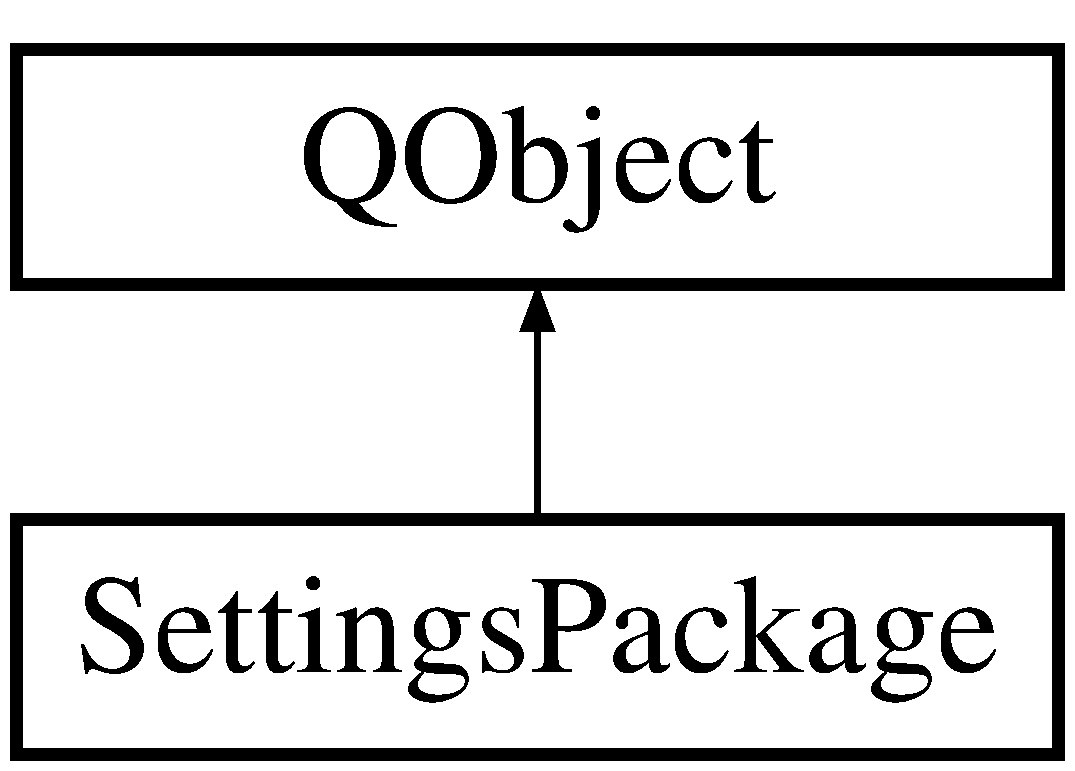
\includegraphics[height=2.000000cm]{class_settings_package}
\end{center}
\end{figure}
\subsection*{Public Member Functions}
\begin{DoxyCompactItemize}
\item 
\hyperlink{class_settings_package_a387aa321903917fad11b1897f7c4d357}{Settings\+Package} ()\hypertarget{class_settings_package_a387aa321903917fad11b1897f7c4d357}{}\label{class_settings_package_a387aa321903917fad11b1897f7c4d357}

\begin{DoxyCompactList}\small\item\em Default \hyperlink{class_settings_package}{Settings\+Package} Constructor, calls default constructors for a Graphics, Optimizer and Problem\+Domain \hyperlink{class_settings_package}{Settings\+Package}. \end{DoxyCompactList}\item 
\hyperlink{class_graphics_settings_package}{Graphics\+Settings\+Package} $\ast$ \hyperlink{class_settings_package_a7eb1432a2fbda1d204ef73b47b46d1e2}{get\+Graphics\+Settings\+Package} ()
\item 
\hyperlink{class_optimizer_settings_package}{Optimizer\+Settings\+Package} $\ast$ \hyperlink{class_settings_package_a6fa4b42272cf9c8d3847c038bf591914}{get\+Optimizer\+Settings\+Package} ()
\item 
\hyperlink{class_problem_domain_settings_package}{Problem\+Domain\+Settings\+Package} $\ast$ \hyperlink{class_settings_package_a343a97ef7424b400ab17480b77051466}{get\+Problem\+Domain\+Settings\+Package} ()
\item 
Q\+\_\+\+I\+N\+V\+O\+K\+A\+B\+LE void \hyperlink{class_settings_package_aa2c0392e2df98086e2ef64b640e2aab4}{generate\+Settings\+General} (int)
\begin{DoxyCompactList}\small\item\em Sets the swarm size (given by G\+UI) \end{DoxyCompactList}\item 
Q\+\_\+\+I\+N\+V\+O\+K\+A\+B\+LE void \hyperlink{class_settings_package_a1c2aabf66f20e3240c6e35e9e3385081}{generate\+Settings\+Graphics} (Q\+String, int, bool, bool, int)\hypertarget{class_settings_package_a1c2aabf66f20e3240c6e35e9e3385081}{}\label{class_settings_package_a1c2aabf66f20e3240c6e35e9e3385081}

\begin{DoxyCompactList}\small\item\em Generates a \hyperlink{class_graphics_settings_package}{Graphics\+Settings\+Package} using input from the G\+UI. \end{DoxyCompactList}\item 
Q\+\_\+\+I\+N\+V\+O\+K\+A\+B\+LE void \hyperlink{class_settings_package_abab2f666693f6a074e825ef821f5160a}{generate\+Settings\+Optimizer} (Q\+String $\ast$, double, double, double)\hypertarget{class_settings_package_abab2f666693f6a074e825ef821f5160a}{}\label{class_settings_package_abab2f666693f6a074e825ef821f5160a}

\begin{DoxyCompactList}\small\item\em Generates a \hyperlink{class_optimizer_settings_package}{Optimizer\+Settings\+Package} using input from the G\+UI. \end{DoxyCompactList}\item 
Q\+\_\+\+I\+N\+V\+O\+K\+A\+B\+LE void \hyperlink{class_settings_package_a9e0fa6d7c66966afa3b224977b1be723}{generate\+Settings\+Domain} (Q\+String, int, int, int, int, int, double, double, double)\hypertarget{class_settings_package_a9e0fa6d7c66966afa3b224977b1be723}{}\label{class_settings_package_a9e0fa6d7c66966afa3b224977b1be723}

\begin{DoxyCompactList}\small\item\em Generates a \hyperlink{class_problem_domain_settings_package}{Problem\+Domain\+Settings\+Package} using input from the G\+UI. \end{DoxyCompactList}\end{DoxyCompactItemize}


\subsection{Member Function Documentation}
\index{Settings\+Package@{Settings\+Package}!generate\+Settings\+General@{generate\+Settings\+General}}
\index{generate\+Settings\+General@{generate\+Settings\+General}!Settings\+Package@{Settings\+Package}}
\subsubsection[{\texorpdfstring{generate\+Settings\+General(int)}{generateSettingsGeneral(int)}}]{\setlength{\rightskip}{0pt plus 5cm}void Settings\+Package\+::generate\+Settings\+General (
\begin{DoxyParamCaption}
\item[{int}]{s\+Size}
\end{DoxyParamCaption}
)}\hypertarget{class_settings_package_aa2c0392e2df98086e2ef64b640e2aab4}{}\label{class_settings_package_aa2c0392e2df98086e2ef64b640e2aab4}


Sets the swarm size (given by G\+UI) 


\begin{DoxyParams}{Parameters}
{\em Swarm\+Size} & (int) \\
\hline
\end{DoxyParams}
\index{Settings\+Package@{Settings\+Package}!get\+Graphics\+Settings\+Package@{get\+Graphics\+Settings\+Package}}
\index{get\+Graphics\+Settings\+Package@{get\+Graphics\+Settings\+Package}!Settings\+Package@{Settings\+Package}}
\subsubsection[{\texorpdfstring{get\+Graphics\+Settings\+Package()}{getGraphicsSettingsPackage()}}]{\setlength{\rightskip}{0pt plus 5cm}{\bf Graphics\+Settings\+Package} $\ast$ Settings\+Package\+::get\+Graphics\+Settings\+Package (
\begin{DoxyParamCaption}
{}
\end{DoxyParamCaption}
)}\hypertarget{class_settings_package_a7eb1432a2fbda1d204ef73b47b46d1e2}{}\label{class_settings_package_a7eb1432a2fbda1d204ef73b47b46d1e2}
\begin{DoxyReturn}{Returns}
Returns the associated \hyperlink{class_graphics_settings_package}{Graphics\+Settings\+Package} 
\end{DoxyReturn}
\index{Settings\+Package@{Settings\+Package}!get\+Optimizer\+Settings\+Package@{get\+Optimizer\+Settings\+Package}}
\index{get\+Optimizer\+Settings\+Package@{get\+Optimizer\+Settings\+Package}!Settings\+Package@{Settings\+Package}}
\subsubsection[{\texorpdfstring{get\+Optimizer\+Settings\+Package()}{getOptimizerSettingsPackage()}}]{\setlength{\rightskip}{0pt plus 5cm}{\bf Optimizer\+Settings\+Package} $\ast$ Settings\+Package\+::get\+Optimizer\+Settings\+Package (
\begin{DoxyParamCaption}
{}
\end{DoxyParamCaption}
)}\hypertarget{class_settings_package_a6fa4b42272cf9c8d3847c038bf591914}{}\label{class_settings_package_a6fa4b42272cf9c8d3847c038bf591914}
\begin{DoxyReturn}{Returns}
Returns the associated \hyperlink{class_optimizer_settings_package}{Optimizer\+Settings\+Package} 
\end{DoxyReturn}
\index{Settings\+Package@{Settings\+Package}!get\+Problem\+Domain\+Settings\+Package@{get\+Problem\+Domain\+Settings\+Package}}
\index{get\+Problem\+Domain\+Settings\+Package@{get\+Problem\+Domain\+Settings\+Package}!Settings\+Package@{Settings\+Package}}
\subsubsection[{\texorpdfstring{get\+Problem\+Domain\+Settings\+Package()}{getProblemDomainSettingsPackage()}}]{\setlength{\rightskip}{0pt plus 5cm}{\bf Problem\+Domain\+Settings\+Package} $\ast$ Settings\+Package\+::get\+Problem\+Domain\+Settings\+Package (
\begin{DoxyParamCaption}
{}
\end{DoxyParamCaption}
)}\hypertarget{class_settings_package_a343a97ef7424b400ab17480b77051466}{}\label{class_settings_package_a343a97ef7424b400ab17480b77051466}
\begin{DoxyReturn}{Returns}
Returns the associated \hyperlink{class_problem_domain_settings_package}{Problem\+Domain\+Settings\+Package} 
\end{DoxyReturn}


The documentation for this class was generated from the following files\+:\begin{DoxyCompactItemize}
\item 
Settings\+Package/settingspackage.\+h\item 
Settings\+Package/settingspackage.\+cpp\end{DoxyCompactItemize}

%--- End generated contents ---

% Index
\backmatter
\newpage
\phantomsection
\clearemptydoublepage
\addcontentsline{toc}{chapter}{Index}
\printindex

\end{document}
